%
% Raças de gatos
%

\documentclass[a4paper]{article}

\usepackage{graphicx}
\usepackage{subfig}


% Variables and shortcuts

\graphicspath{{./cats/}}

% Body

\title{Ra\c{c}as de gatos}
\author{Felipe Micaroni Lalli}

\begin{document}

  \maketitle

  \section{Cornish Rex}

  \bf{Pre\c{c}o aproximado:} R\$ 700 (Buscap\'e}.

  \begin{itemize}
    \item Inglaterra
    \item Amoroso, ativo
    \item Adora a fam\'ilia, se d\'a bem com desconhecidos
    \item P\^elo curto e que cai pouco
  \end{itemize}

  \begin{figure}[ht]
    \centering

    \subfloat[][]{
      \label{fig:cornish-rex01}
      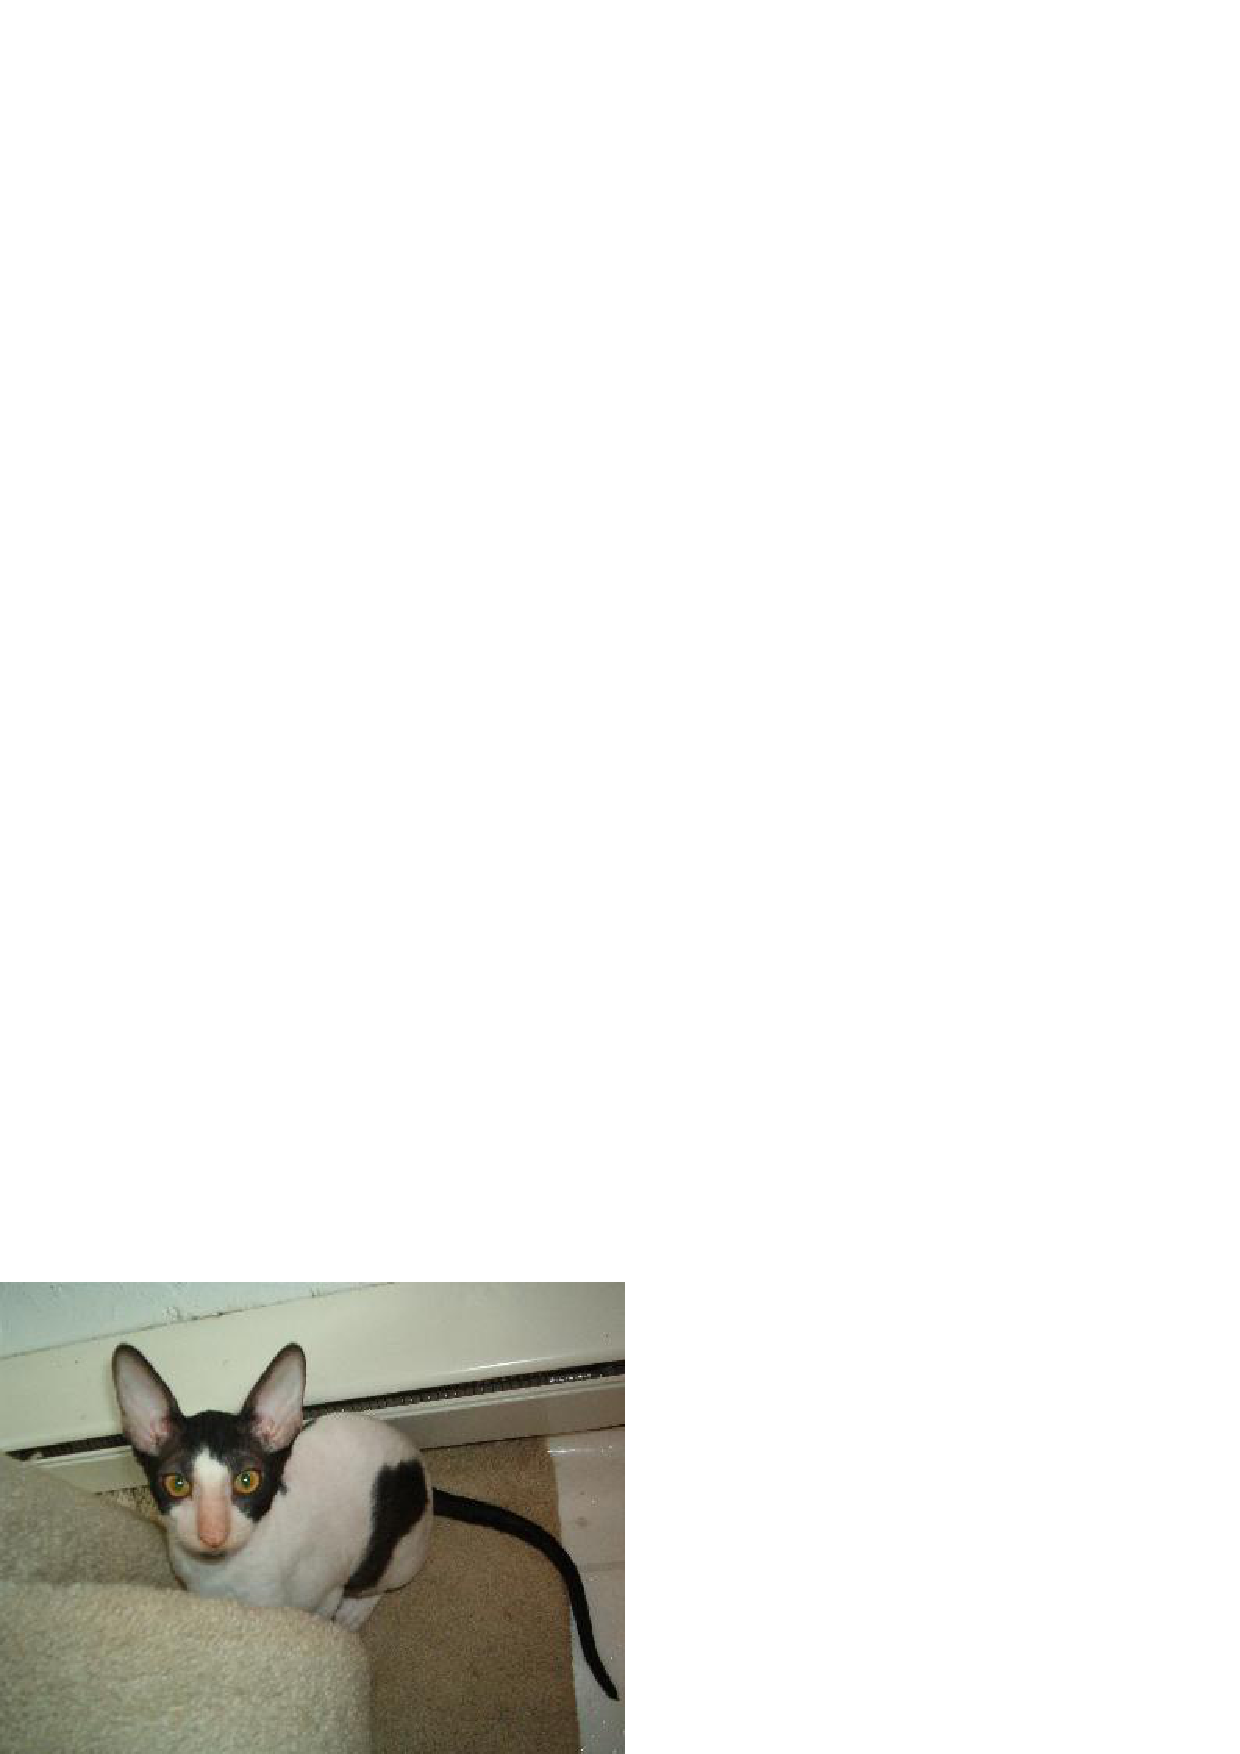
\includegraphics[height=4cm]{cornish-rex01}
    }\subfloat[][Eleg\^ancia de um Cornish Rex]{
      \label{fig:cornish-rex02}
      
\includegraphics[height=4cm]{cornish-rex02}
    }

    \subfloat[][]{
      \label{fig:cornish-rex03}
      
\includegraphics[height=4cm]{cornish-rex03}
    }\subfloat[][Filhotinhos]{
      \label{fig:cornish-rex04}
      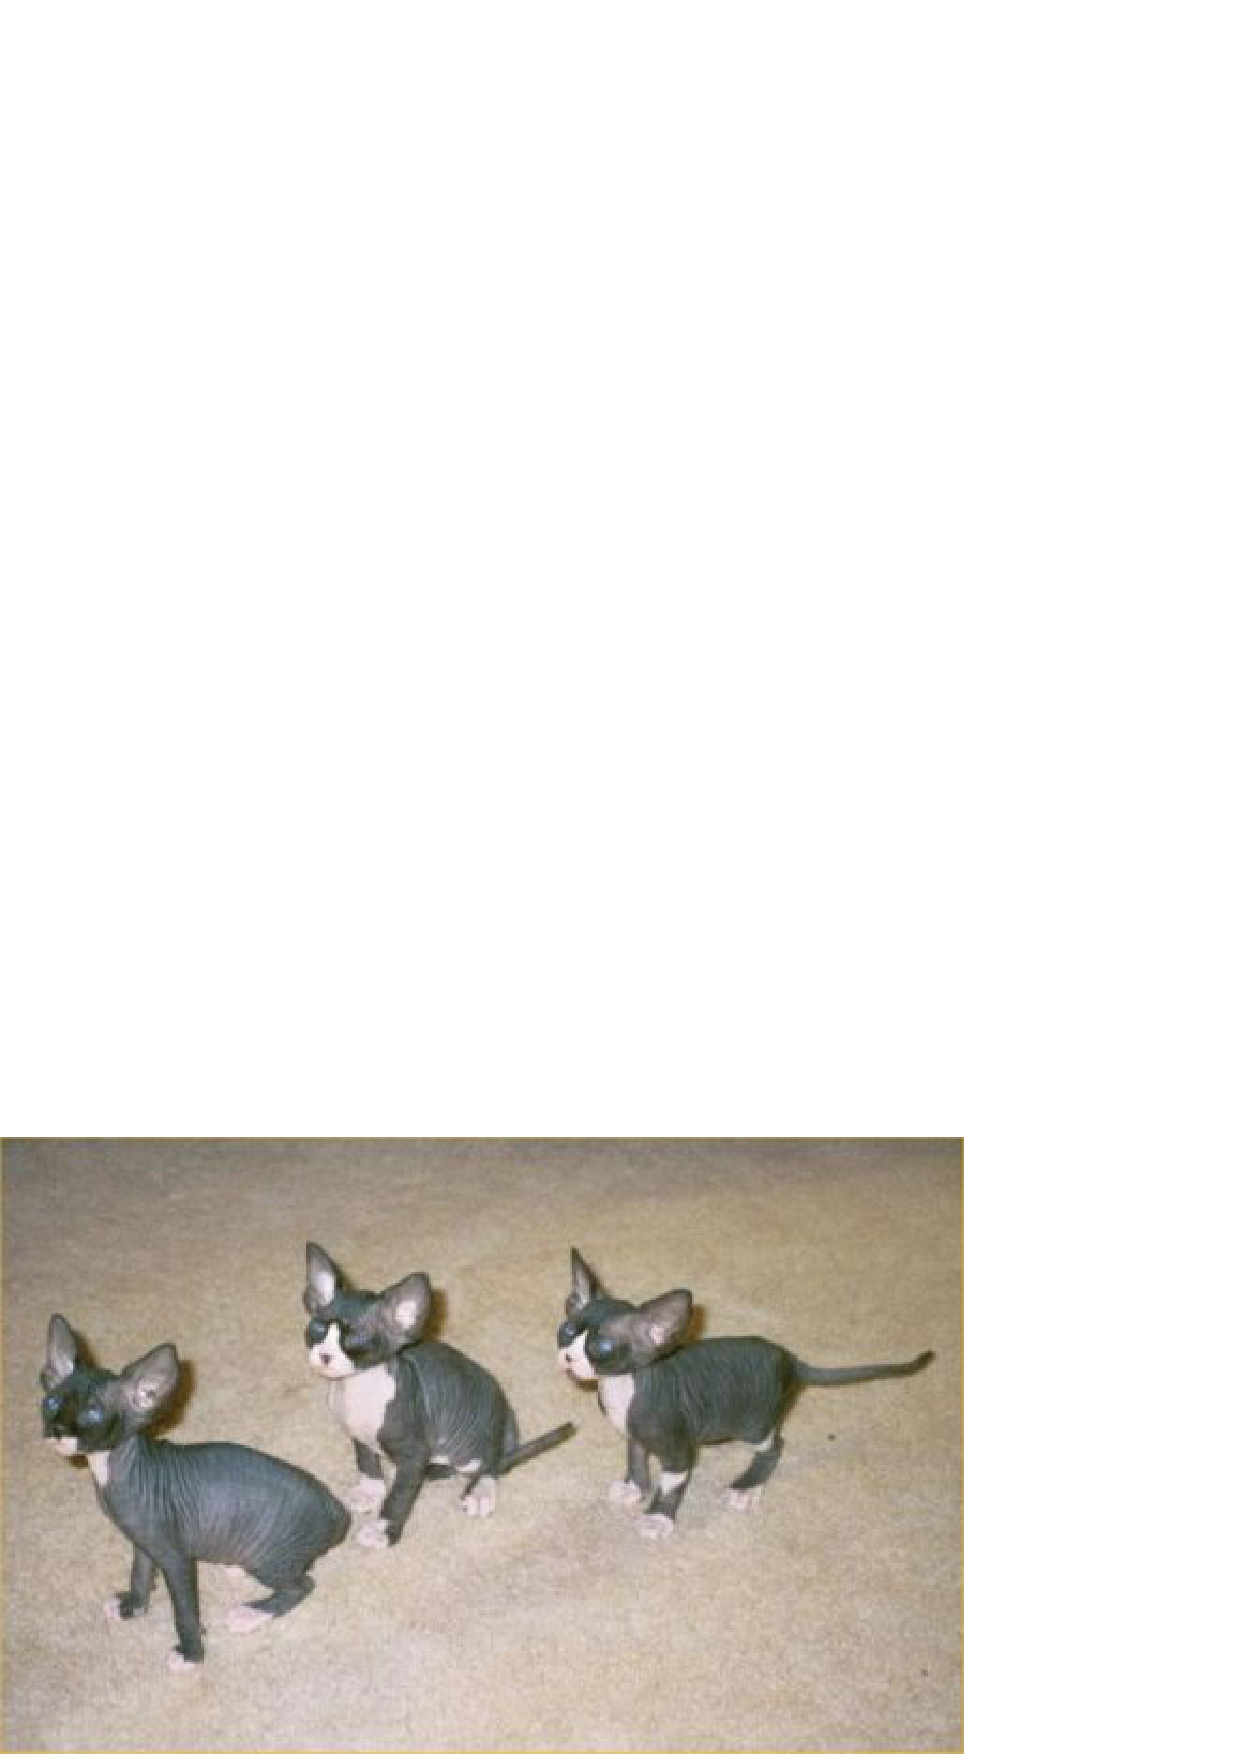
\includegraphics[height=4cm]{cornish-rex04}
    }

    \caption{Exemplares de Cornish Rex}
    \label{fig:cornish-rex}
  \end{figure}
  
  \section{Devon Rex}

  \bf{Pre\c{c}o aproximado:} ?

  \begin{itemize}
    \item Inglaterra
    \item Muito inteligente e d\'a aten\c{c}\~ao \`as pessoas
    \item Pulam muito alto e gostam de espa\c{c}os grandes
  \end{itemize}

  \begin{figure}[ht]
    \centering

    \subfloat[][]{
      \label{fig:devon-rex01}
      
\includegraphics[height=4cm]{devon-rex01}
    }\subfloat[][]{
      \label{fig:devon-rex02}
      
\includegraphics[height=4cm]{devon-rex02}
    }\subfloat[][]{
      \label{fig:devon-rex03}
      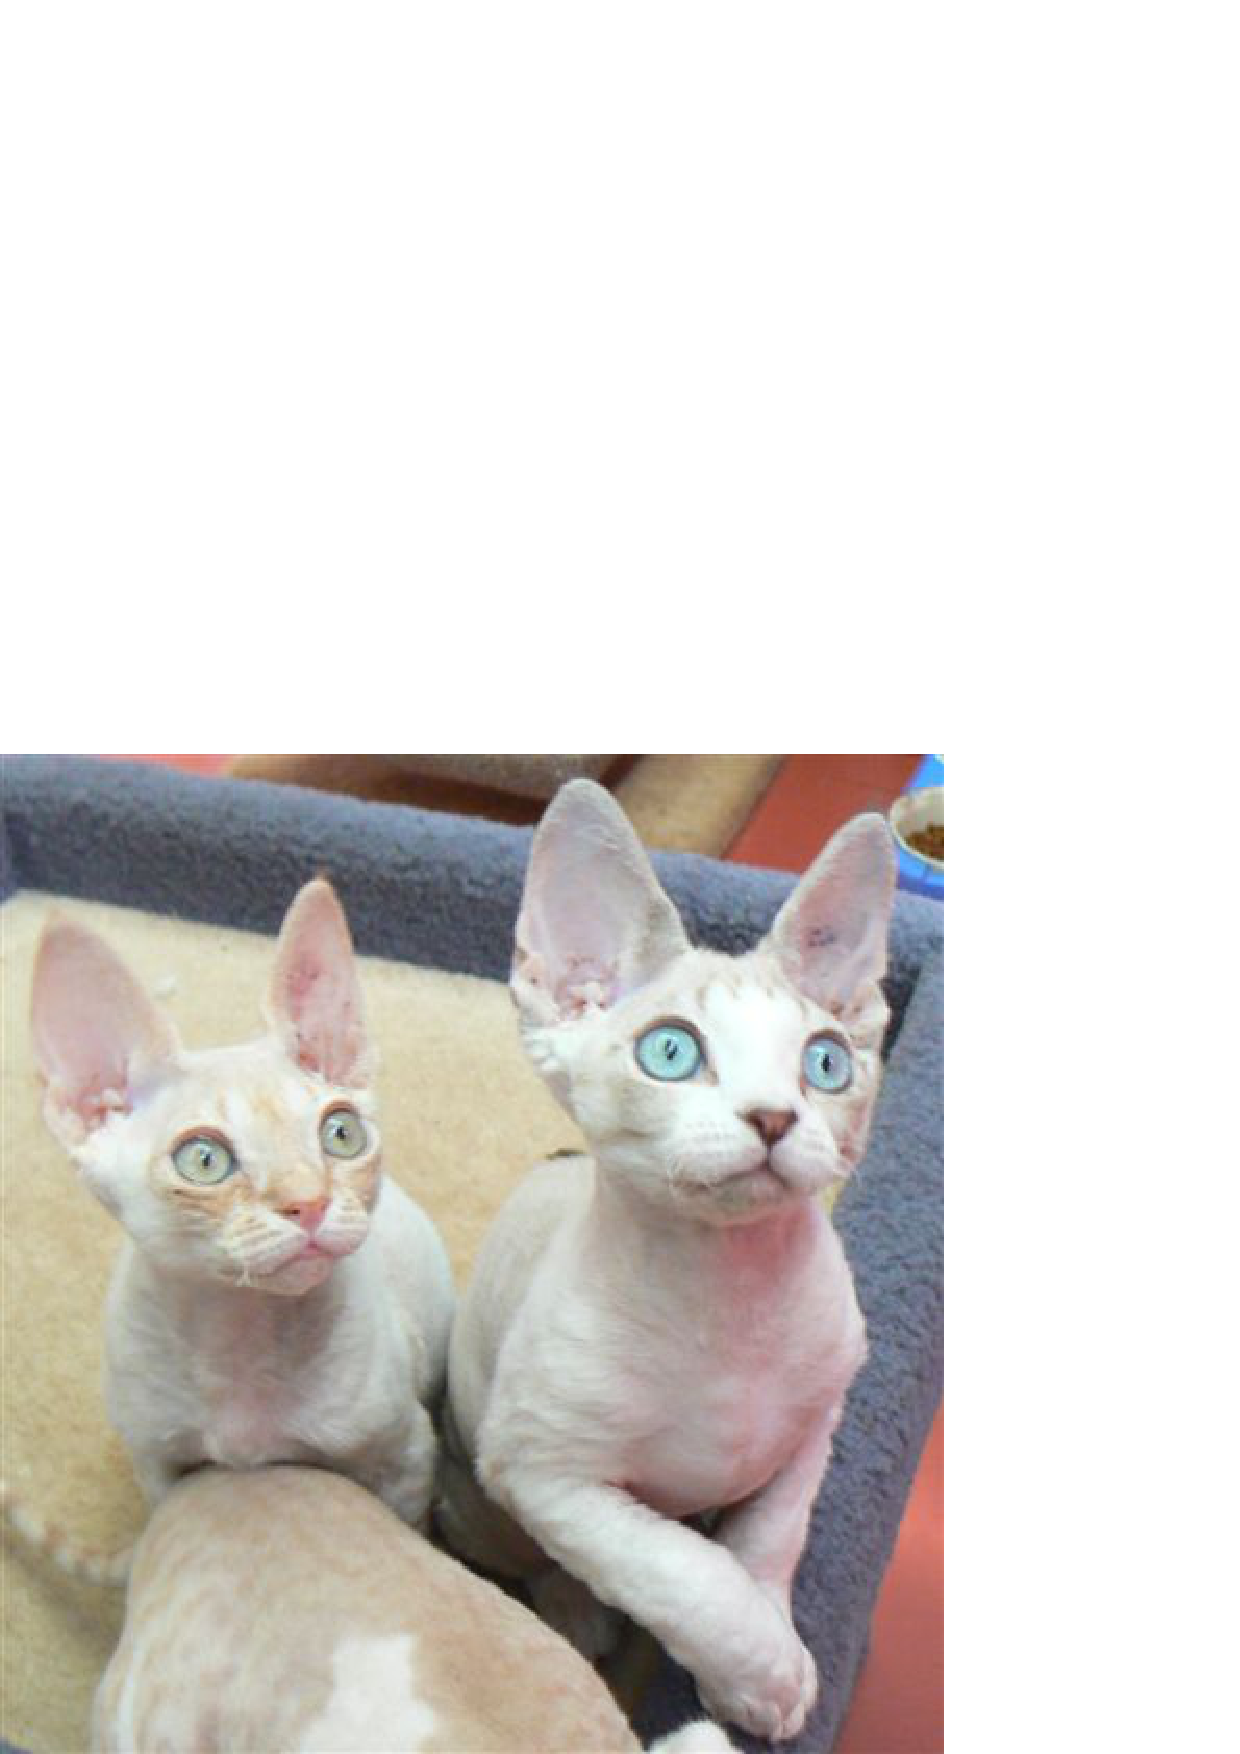
\includegraphics[height=4cm]{devon-rex03}
    }

    \caption{Exemplares de Devon Rex}
    \label{fig:devon-rex}
  \end{figure}

  \section{Korat}

  \bf{Pre\c{c}o aproximado:} ?

  \begin{itemize}
    \item Tail\^andia
    \item P\^elo grosso
    \item Se adapta bem a apartamento
    \item Gosta de fazer companhia para o dono
  \end{itemize}

  \begin{figure}[ht]
    \centering

    \subfloat[][]{
      \label{fig:korat01}
      
\includegraphics[height=4cm]{korat01}
    }\subfloat[][]{
      \label{fig:korat02}
      
\includegraphics[height=4cm]{korat02}
    }

    \caption{Exemplares de Korat}
    \label{fig:korat}
  \end{figure}

  \section{Sphynx}

  \bf{Pre\c{c}o aproximado:} Acima de R\$ 1.500

  \begin{itemize}
    \item Canad\'a
    \item Arisco, \'agil por\'em fiel ao dono
    \item N\~ao vive bem sozinho
    \item Bom em ambientes internos, resistente e saud\'avel
  \end{itemize}

  \begin{figure}[ht]
    \centering

    \subfloat[][]{
      \label{fig:sphynx01}
      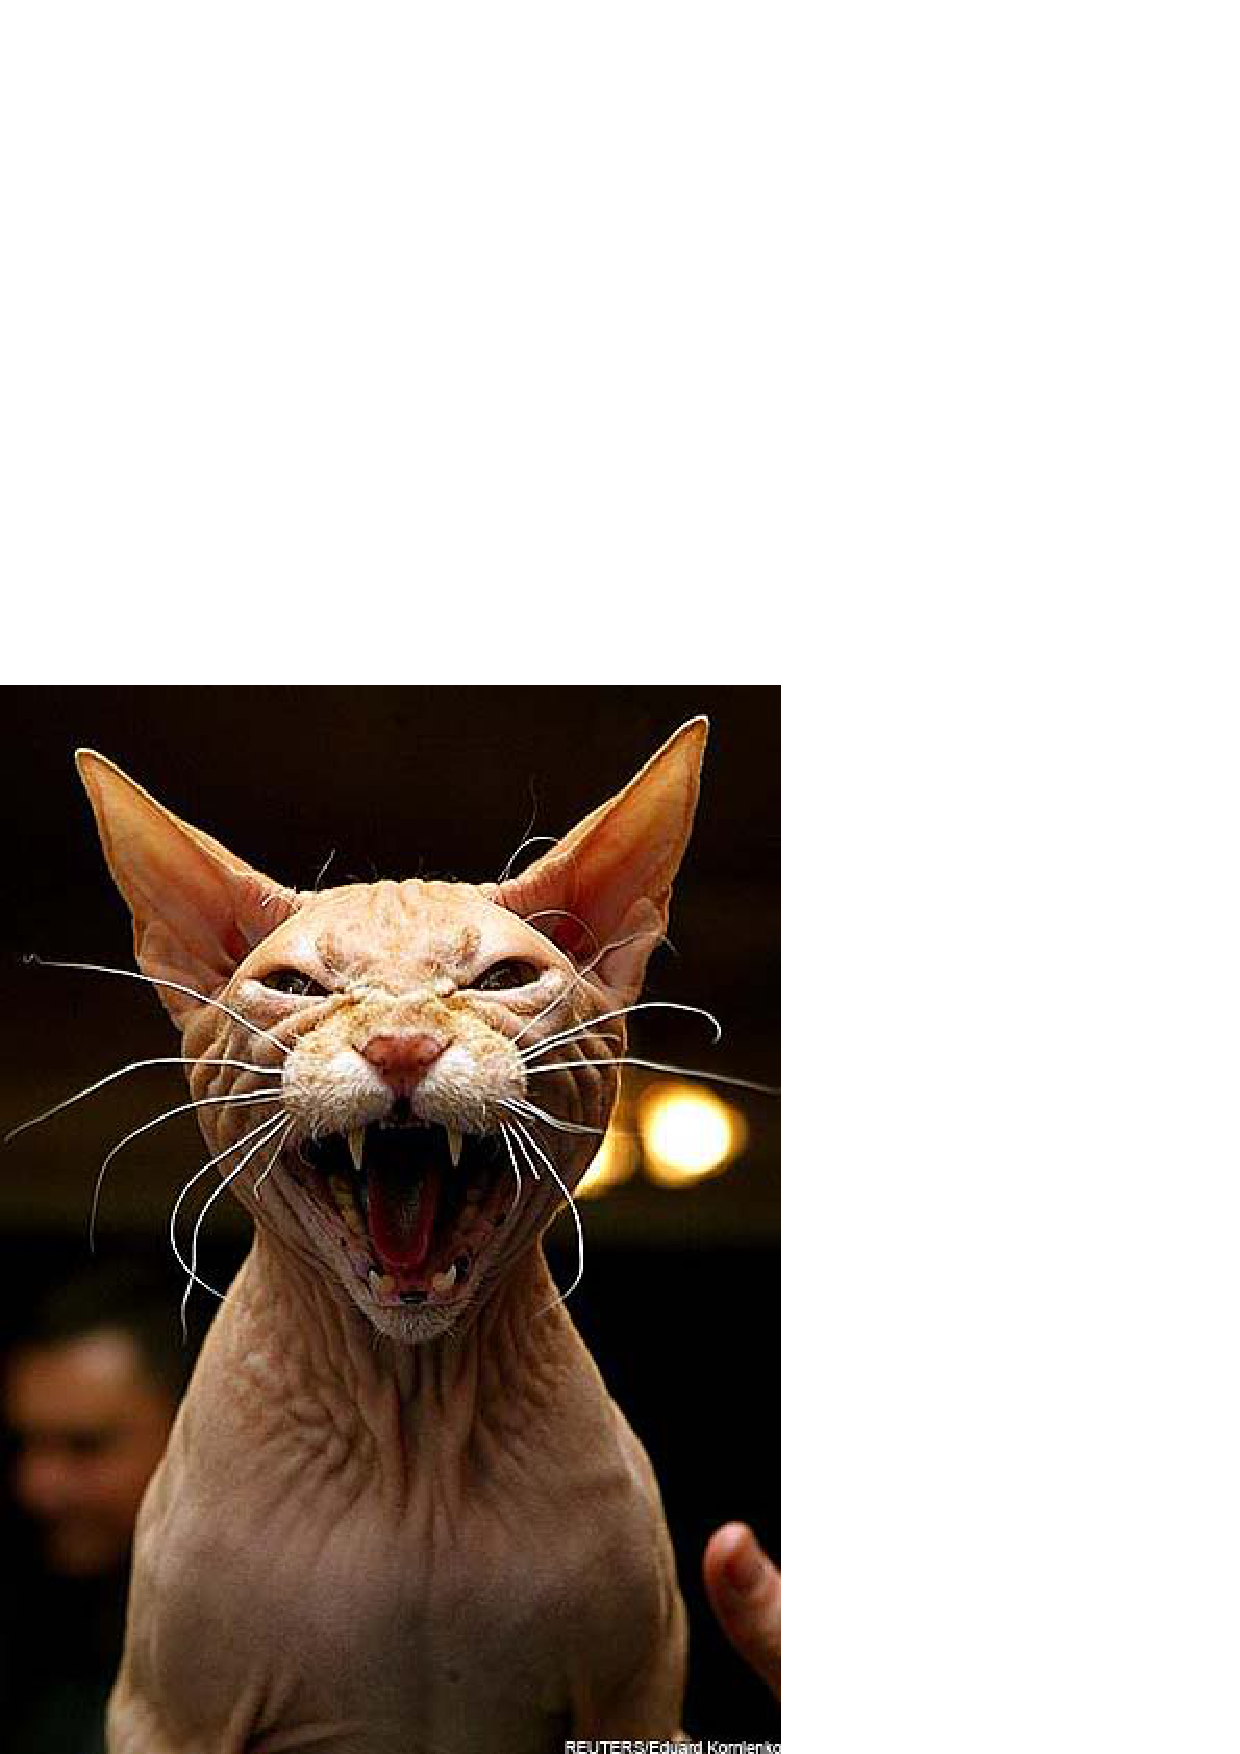
\includegraphics[height=4cm]{sphynx01}
    }\subfloat[][]{
      \label{fig:sphynx02}
      
\includegraphics[height=4cm]{sphynx02}
    }

    \subfloat[][]{
      \label{fig:sphynx03}
      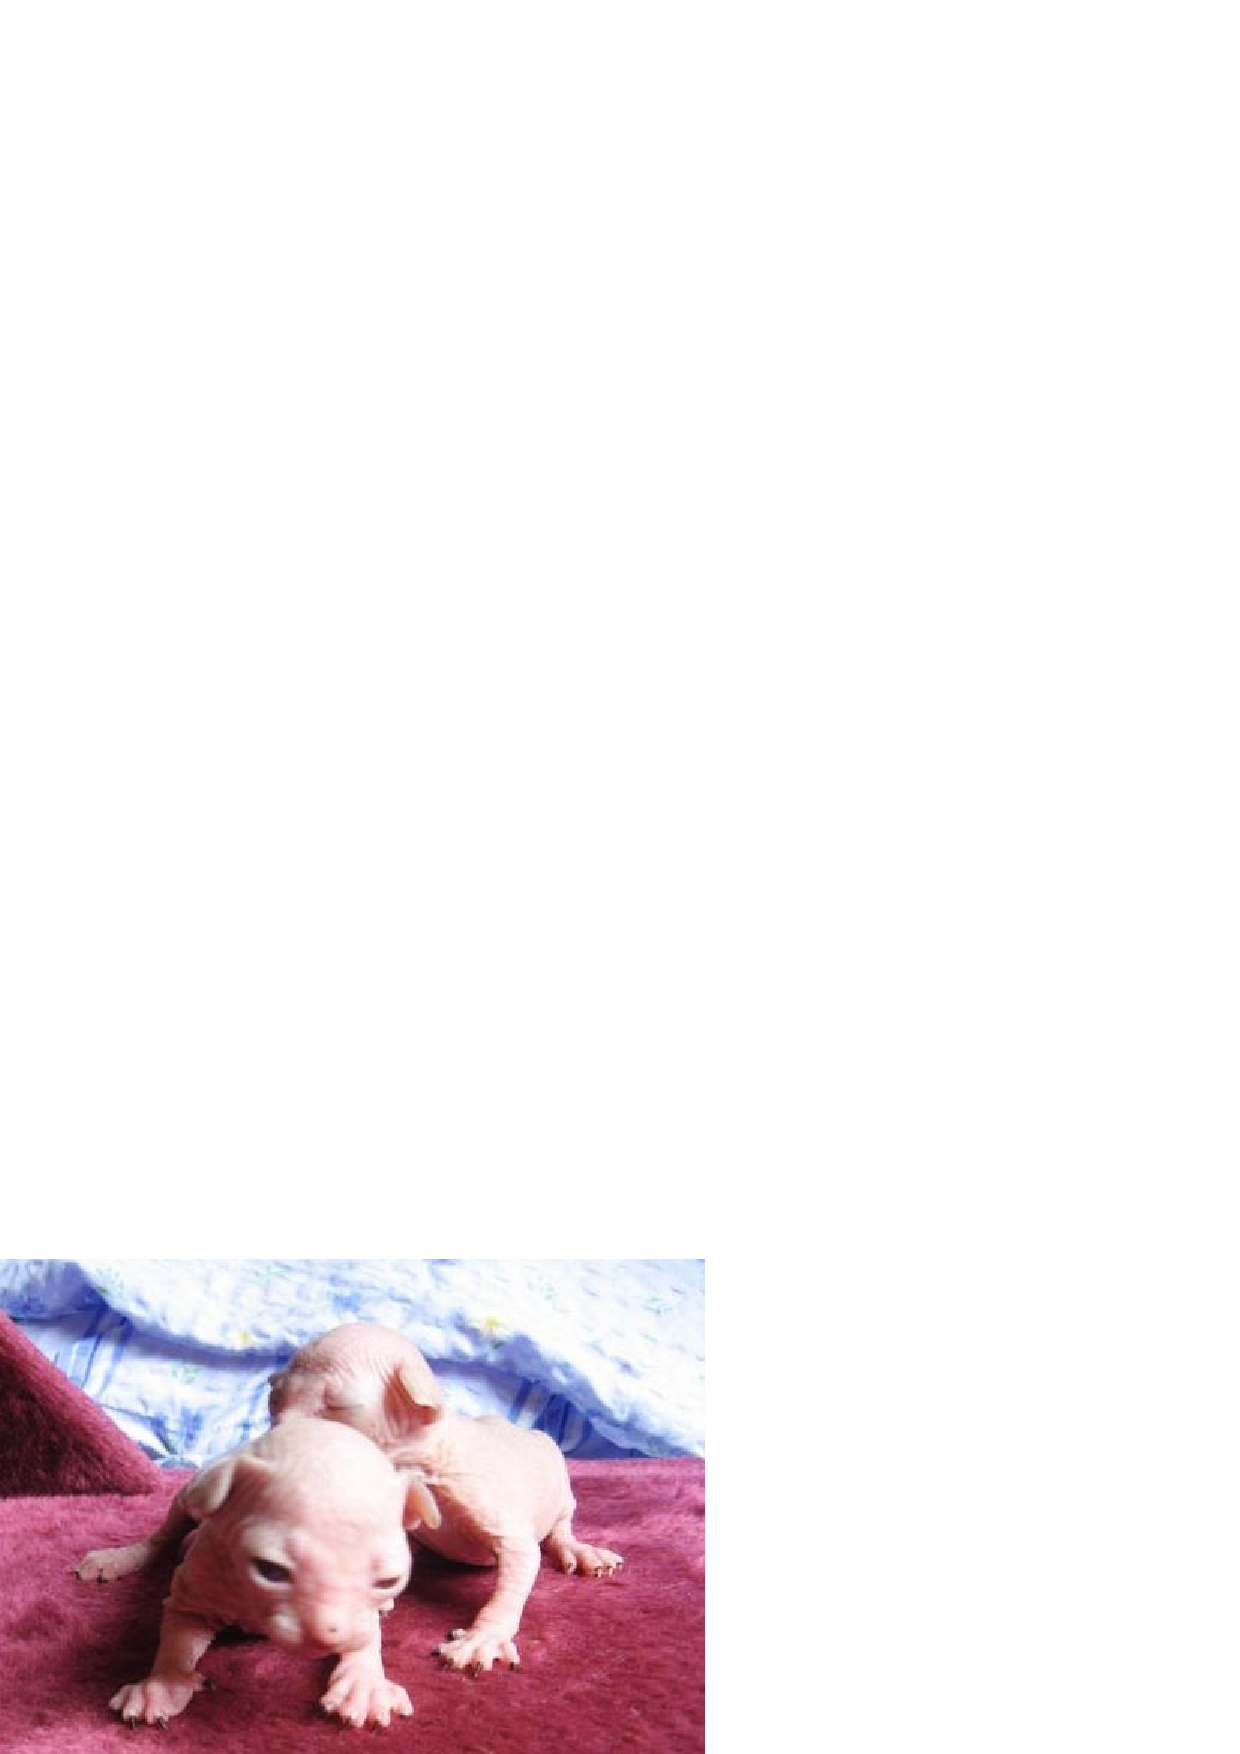
\includegraphics[height=4cm]{sphynx03}
    } \subfloat[][]{
      \label{fig:sphynx04}
      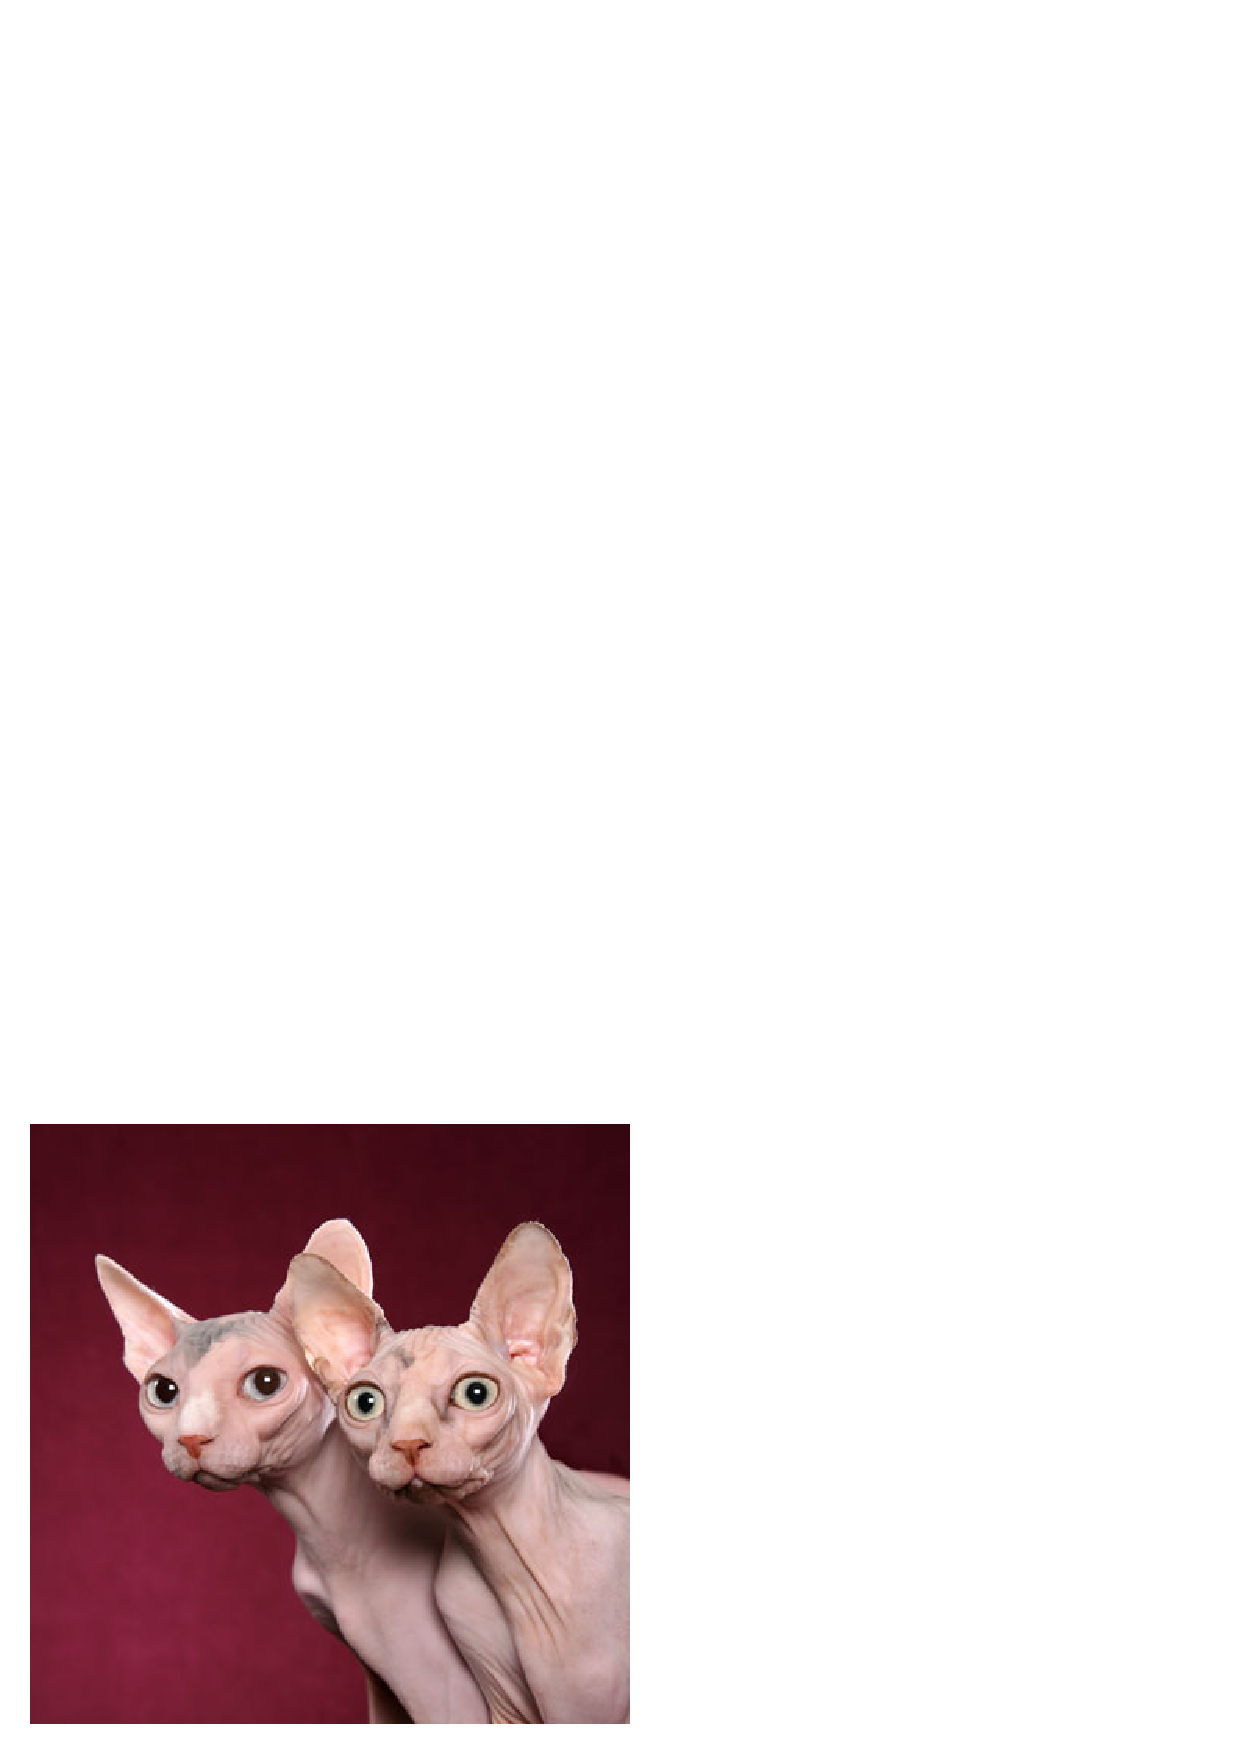
\includegraphics[height=4cm]{sphynx04}
    }

    \caption{Exemplares de Sphynx}
    \label{fig:sphynx}
  \end{figure}

  \section{Peterbald}

  \bf{Pre\c{c}o aproximado:} ?

  \begin{itemize}
    \item R\'ussia
    \item D\'oceis e seguem o dono
  \end{itemize}

  \begin{figure}[ht]
    \centering

    \subfloat[][]{
      \label{fig:peterbald01}
      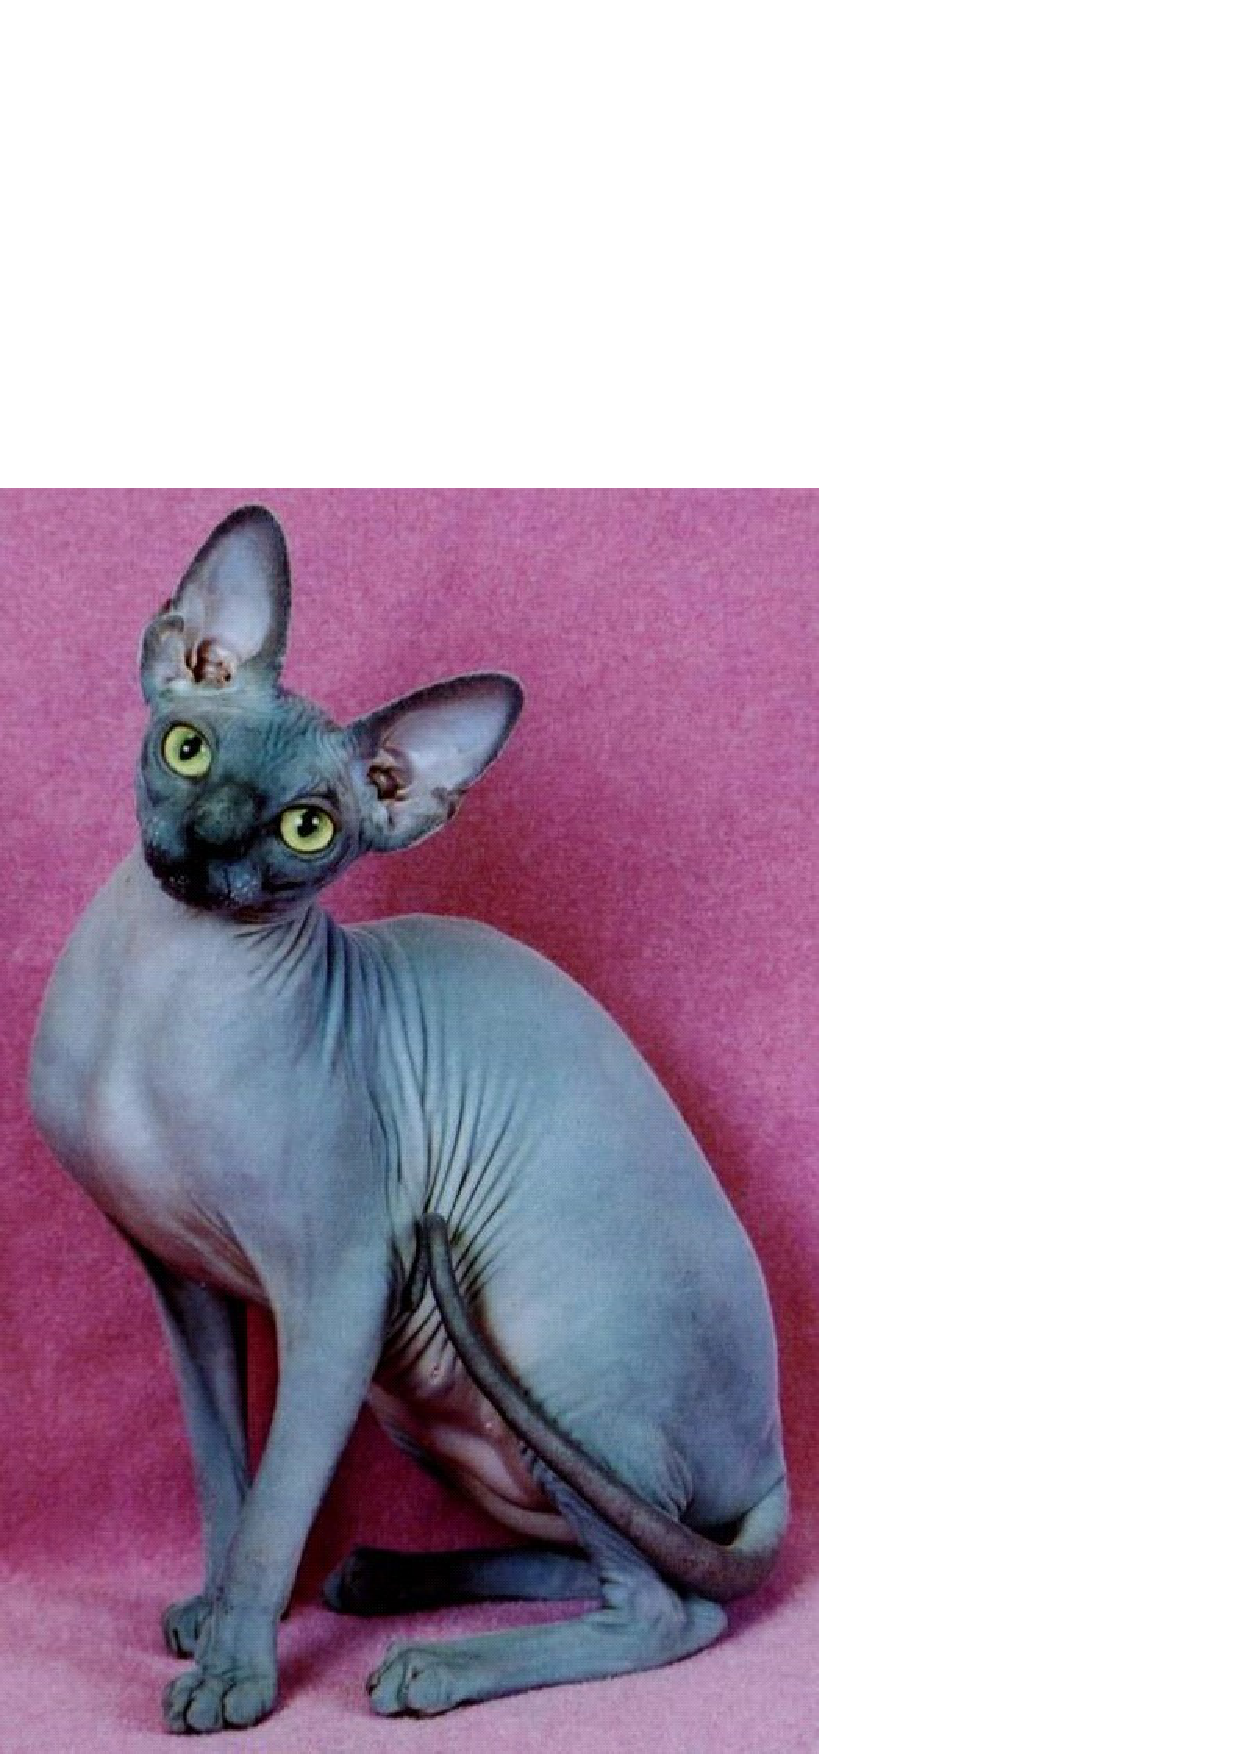
\includegraphics[height=4cm]{peterbald01}
    }\subfloat[][]{
      \label{fig:peterbald02}
      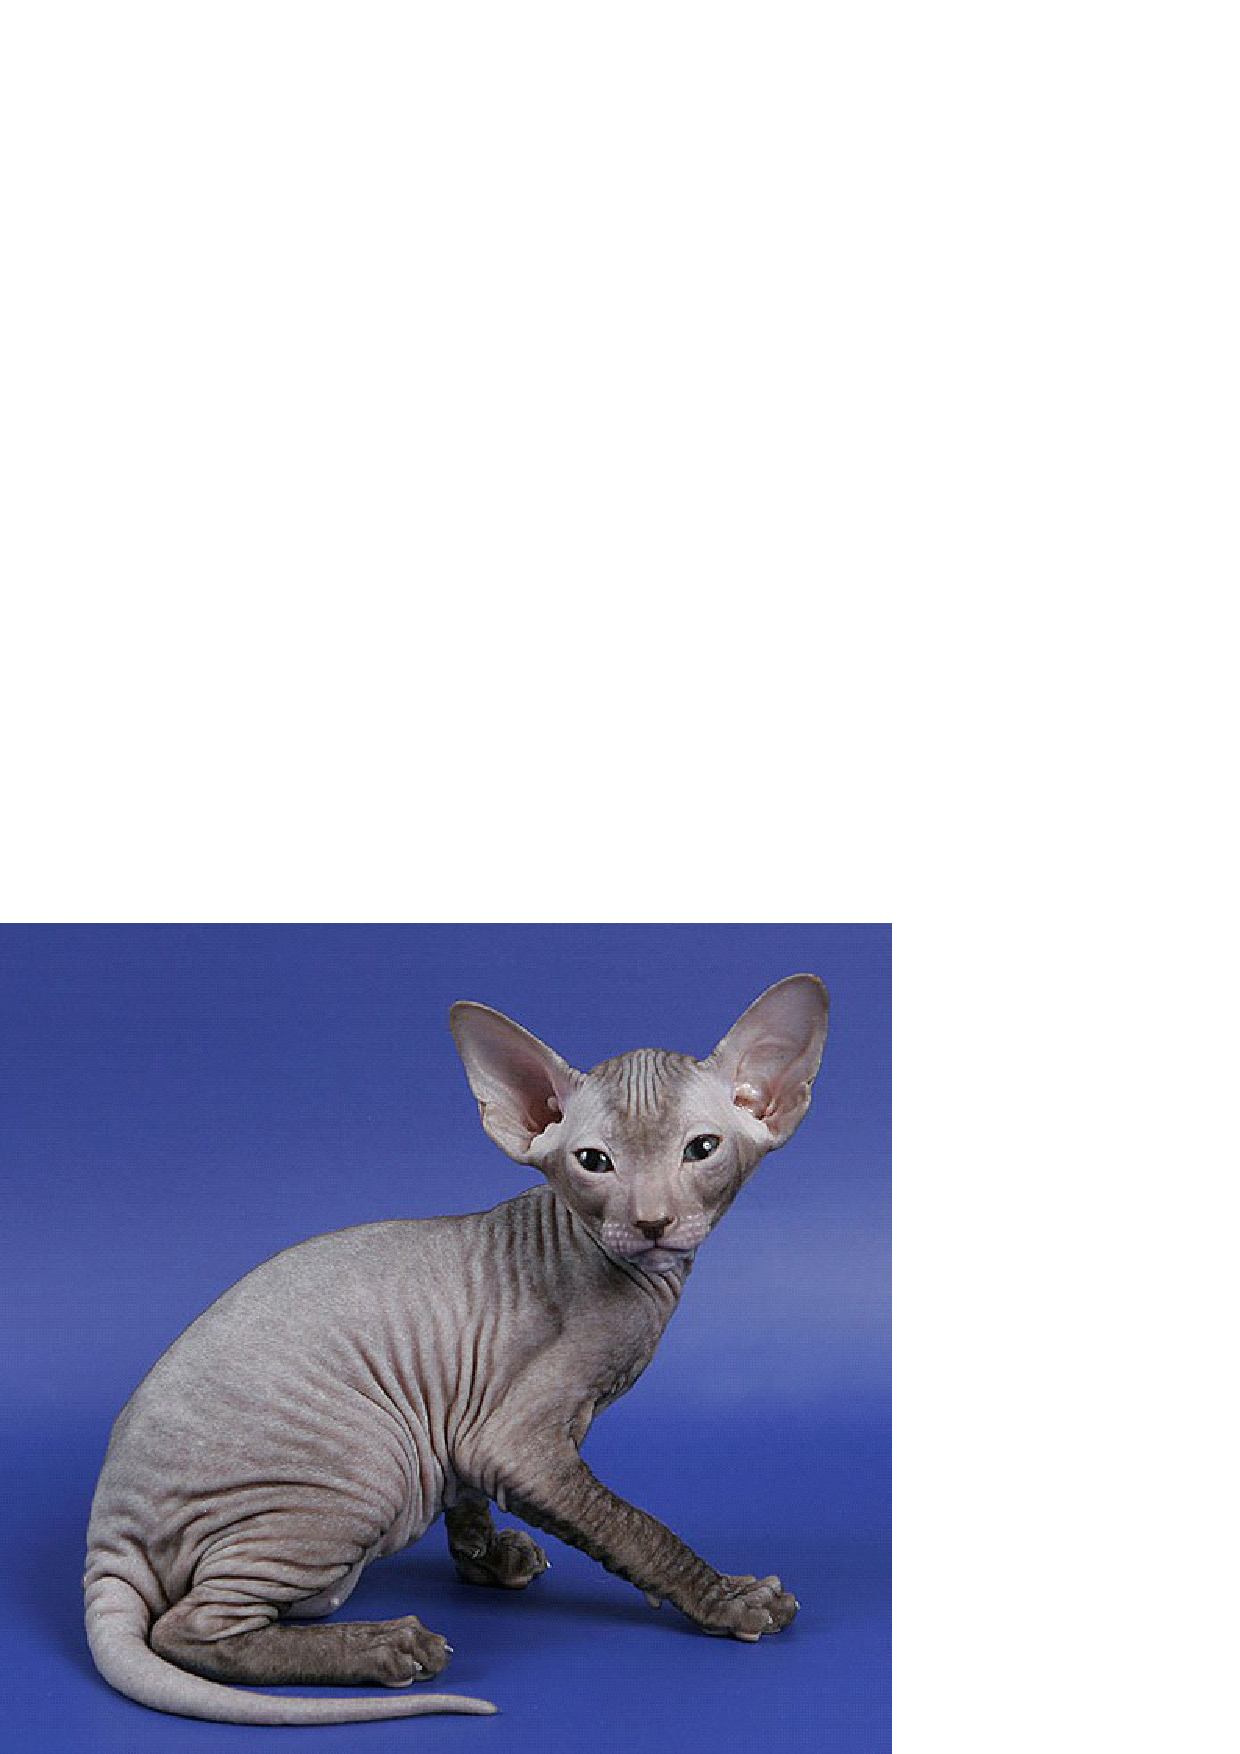
\includegraphics[height=4cm]{peterbald02}
    }

    \subfloat[][]{
      \label{fig:peterbald03}
      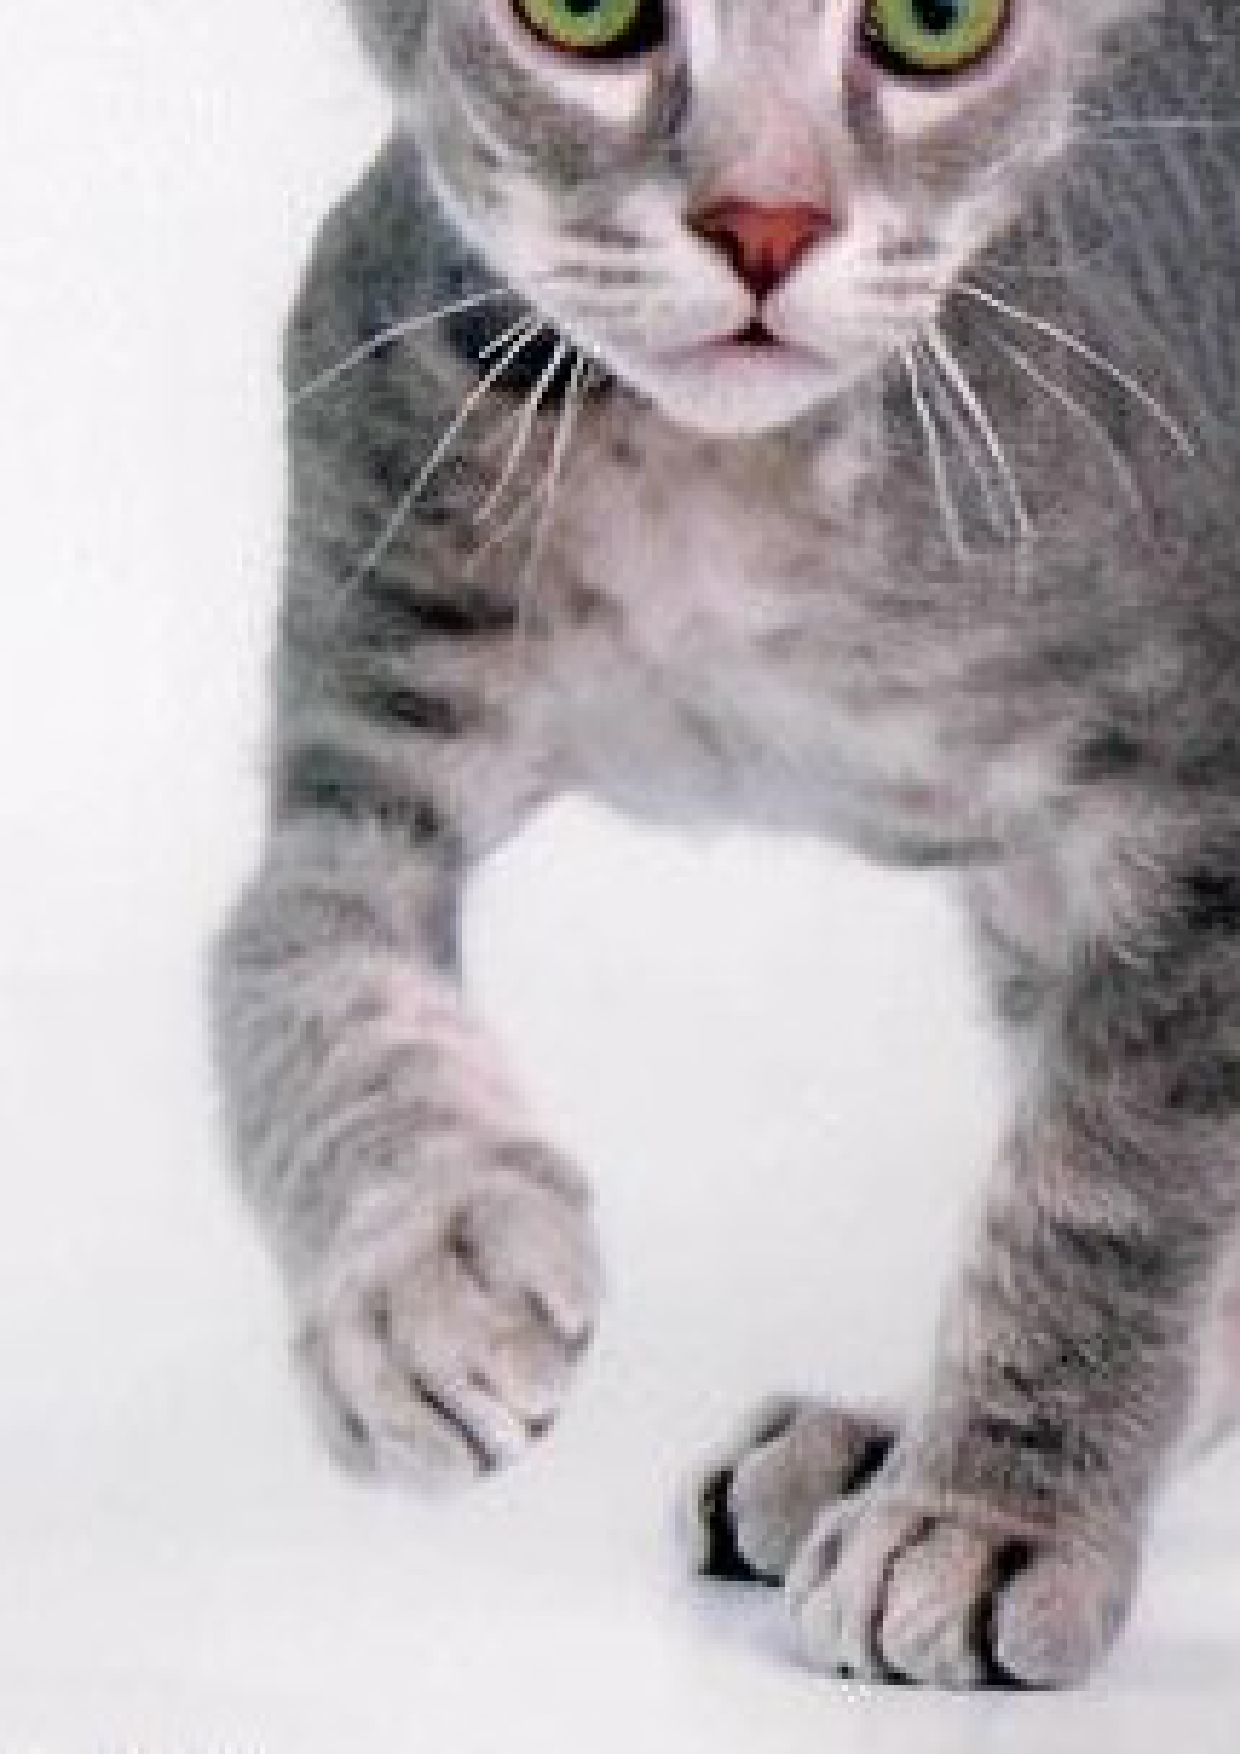
\includegraphics[height=4cm]{peterbald03}
    } \subfloat[][]{
      \label{fig:peterbald04}
      
\includegraphics[height=4cm]{peterbald04}
    } \subfloat[][]{
      \label{fig:peterbald05}
      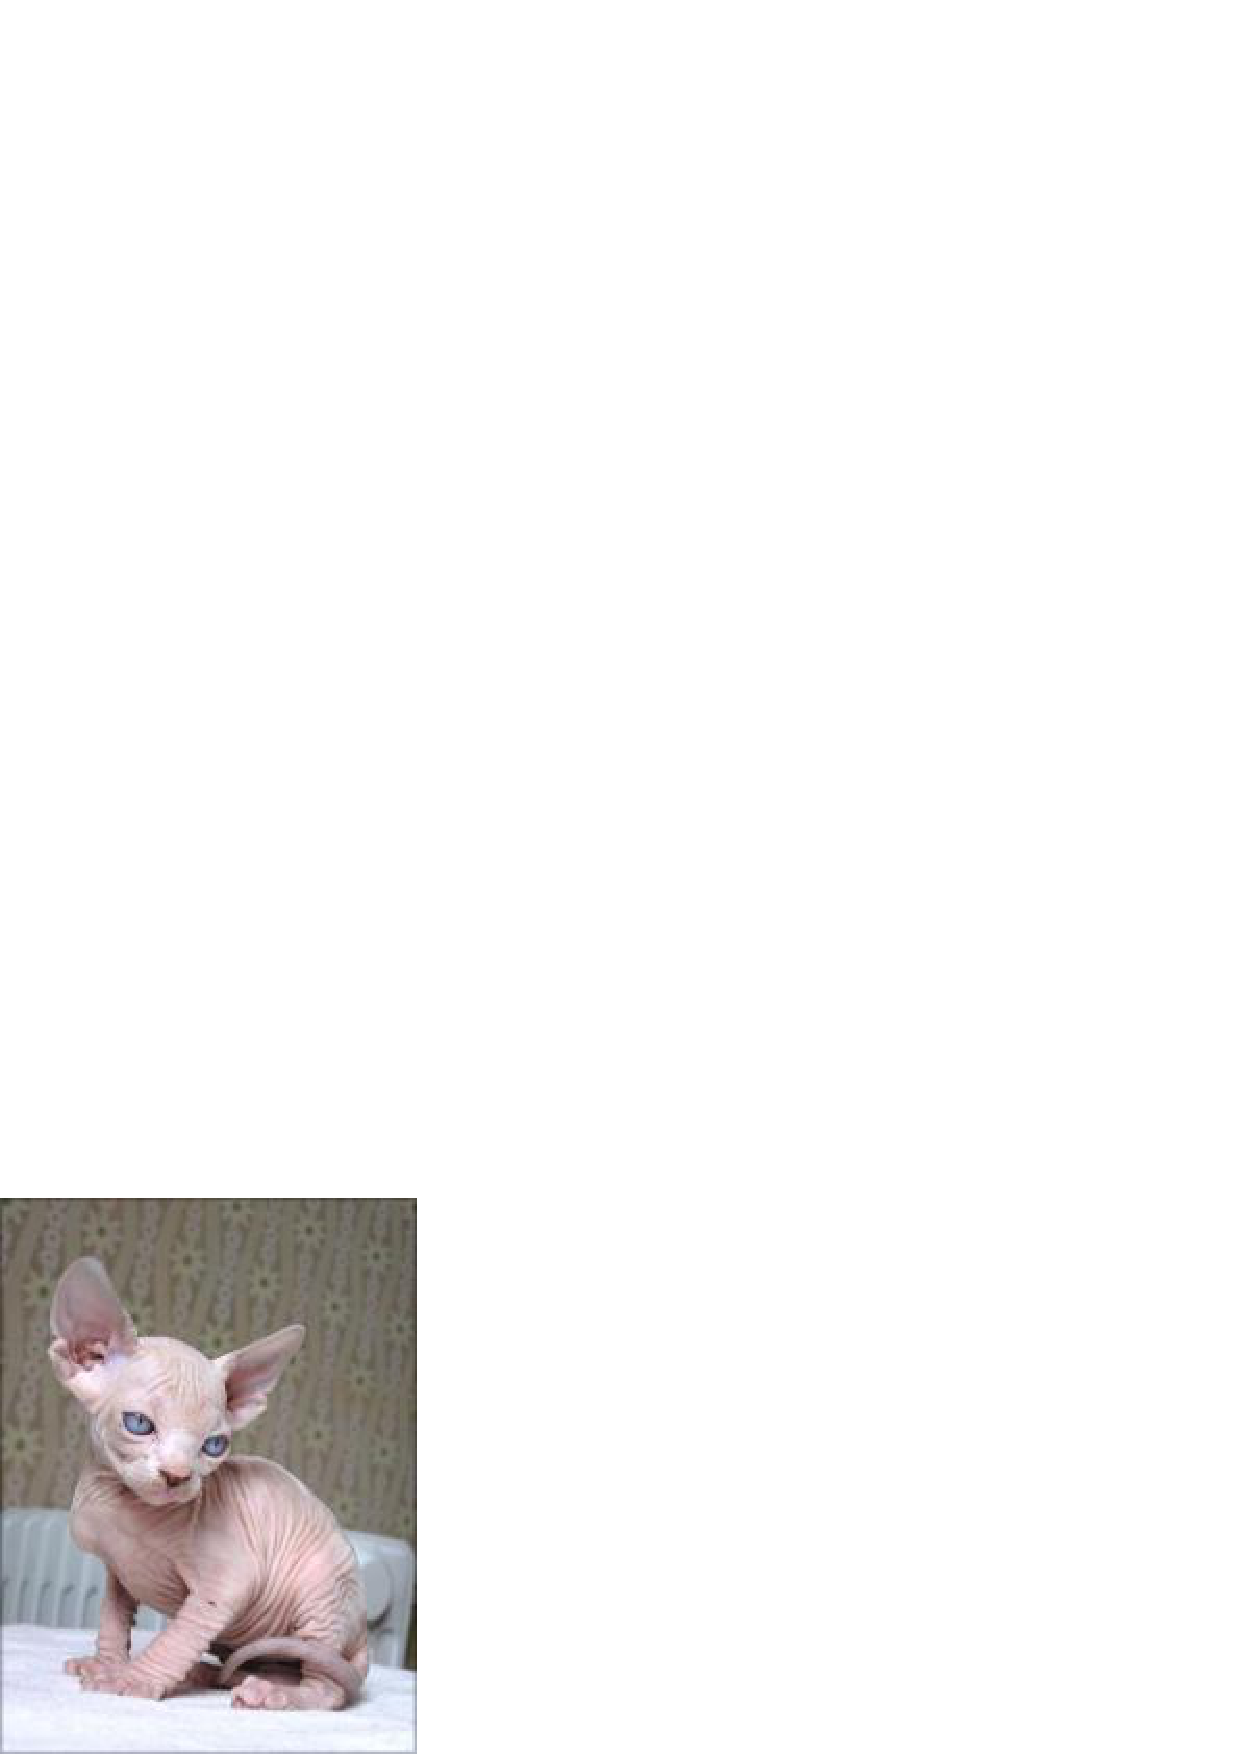
\includegraphics[height=4cm]{peterbald05}
    }

    \caption{Exemplares de Peterbald}
    \label{fig:peterbald}
  \end{figure}

  \section{Maine Coon}

  \bf{Pre\c{c}o aproximado:} R\$ 1.800 a R\$ 3.000

  \begin{itemize}
    \item Estados Unidos da Am\'erica
    \item D\'ocil, meigo, carente de aten\c{c}\~ao
    \item Miado como o de um grilo
  \end{itemize}

  \begin{figure}[ht]
    \centering

    \subfloat[][]{
      \label{fig:maine-coon01}
      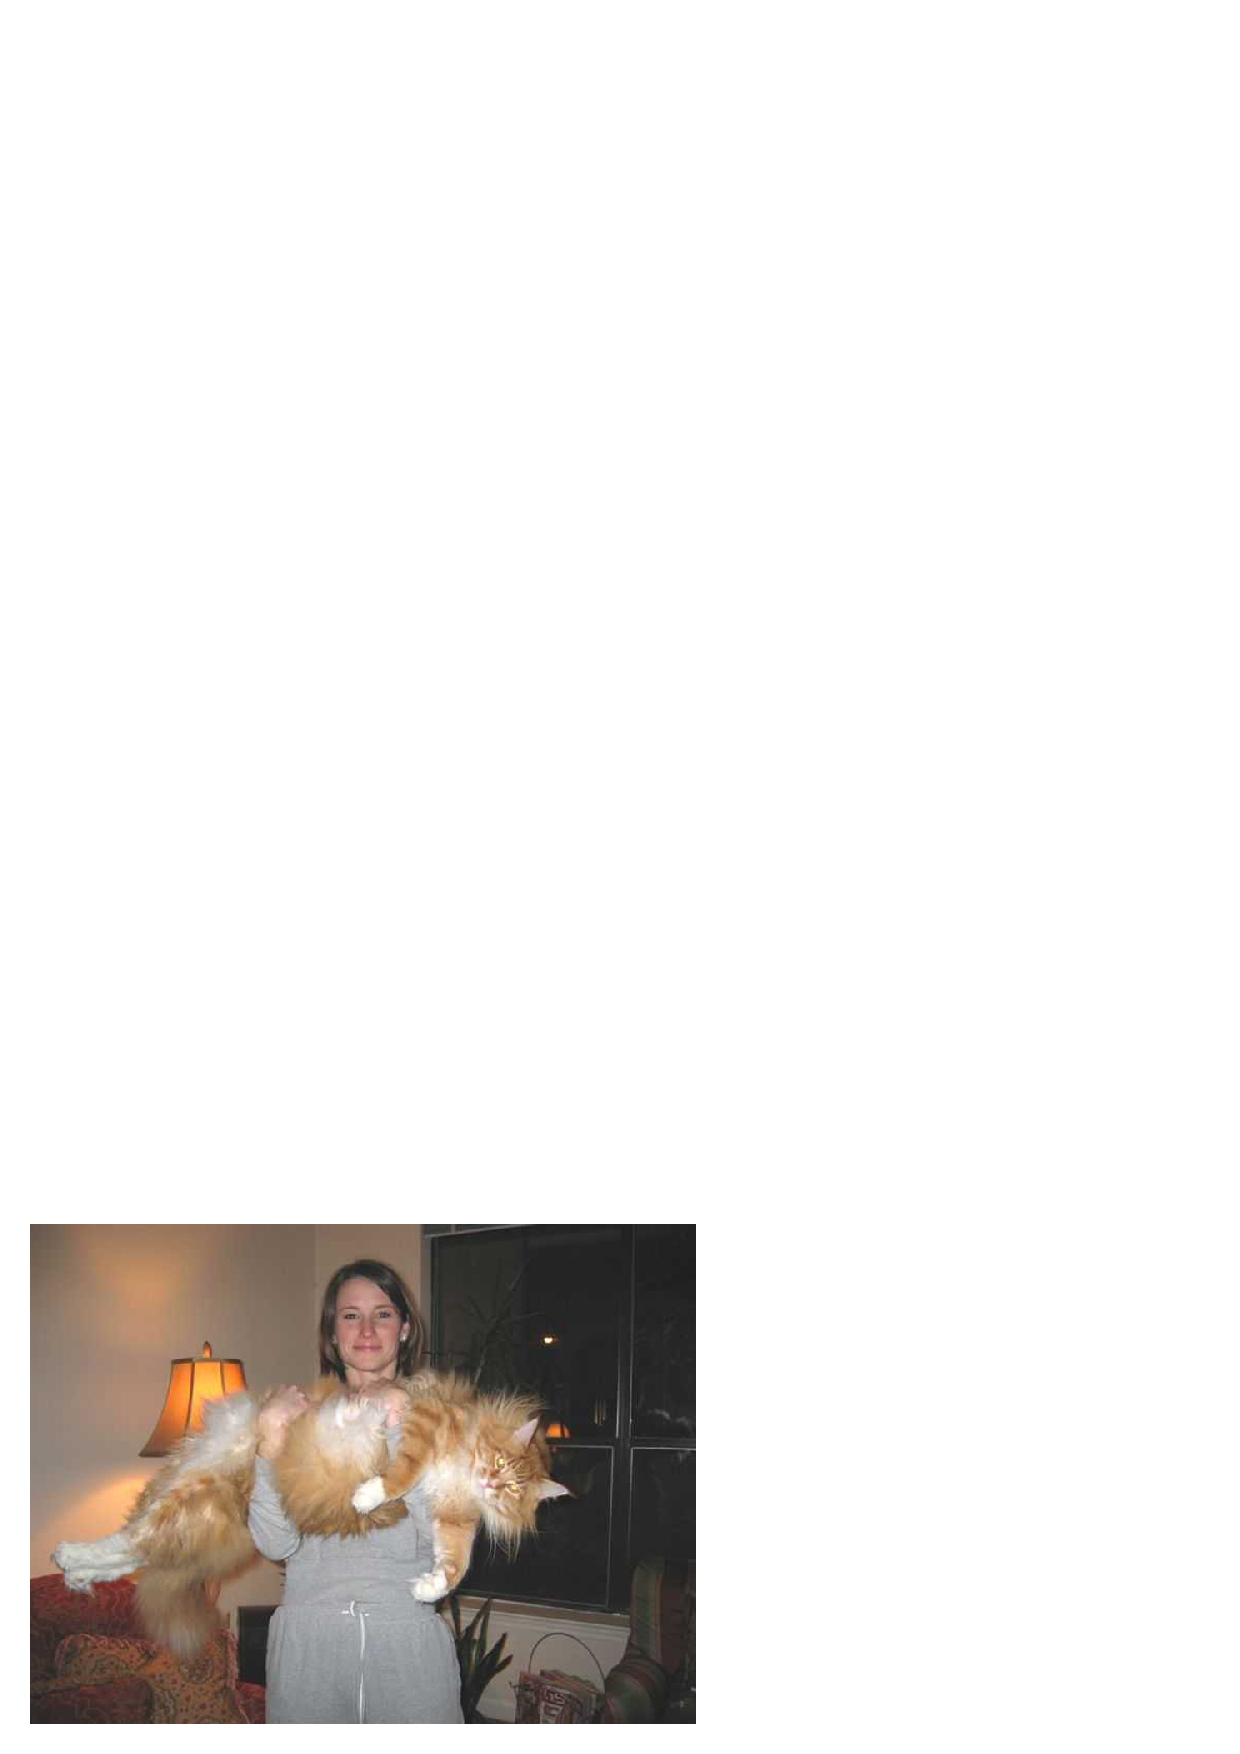
\includegraphics[height=4cm]{maine-coon01}
    } \subfloat[][]{
      \label{fig:maine-coon02}
      \includegraphics[height=4cm]{maine-coon02}
    } \subfloat[][]{
      \label{fig:maine-coon03}
      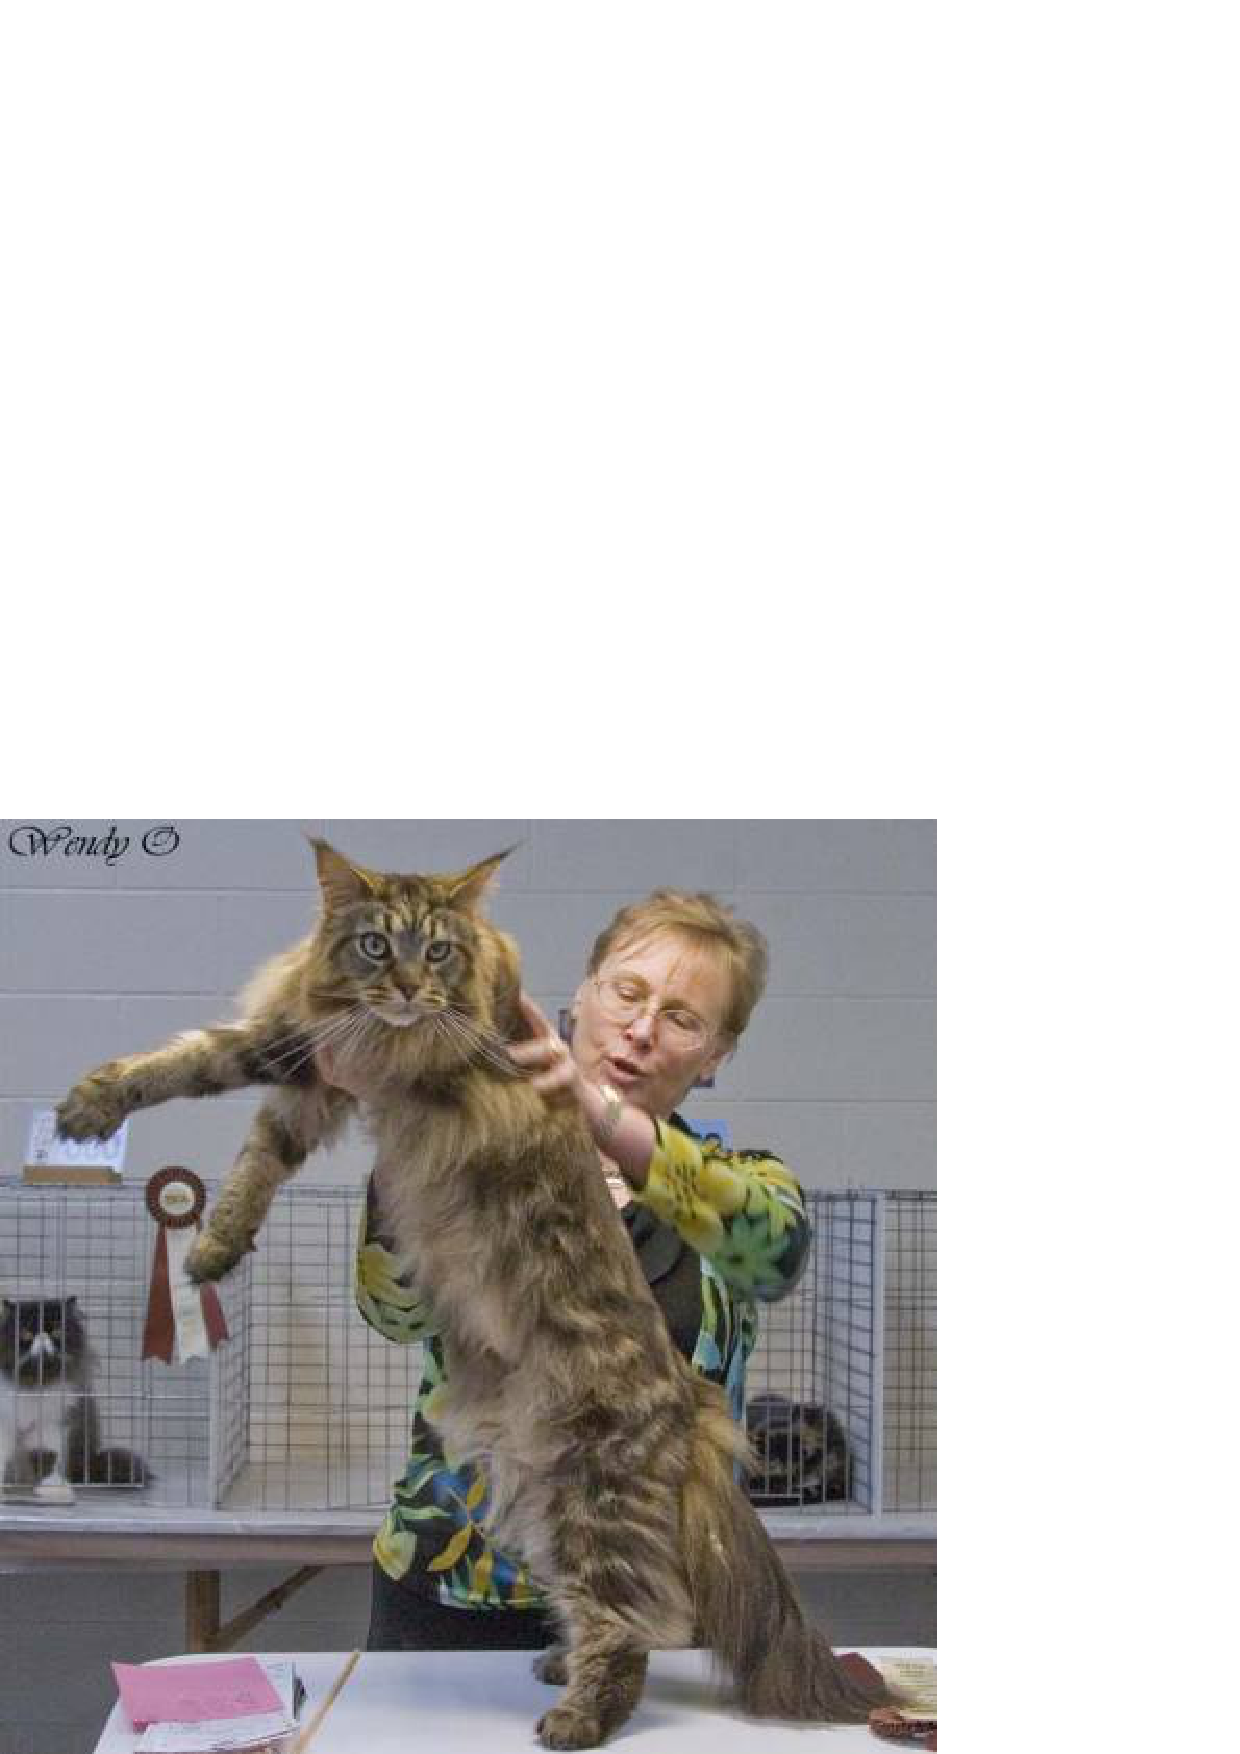
\includegraphics[height=4cm]{maine-coon03}
    }

    \caption{Exemplares de Maine Coon}
    \label{fig:maine-coon}
  \end{figure}


\end{document}
